\documentclass[runningheads,a4paper]{llncs}

\usepackage{amssymb}
\setcounter{tocdepth}{3}
\usepackage{graphicx}
\usepackage{tikz}
\usetikzlibrary{arrows,chains,positioning,scopes,quotes}

\newcommand{\keywords}[1]{\par\addvspace\baselineskip
\noindent\keywordname\endspace\ignorespaces#1}
\pagestyle{plain}

\begin{document}
\def \SystemName {Worlds} % Lol because this shit probably will change.

\mainmatter  % start of an individual contribution

% This needs some work, big time.
\title{\SystemName: A protocol for a distributed P2P MMORPG}

\author{Ryan Walker\\
				Ryan.cjw@gmail.com\\
				\~wlkr}

\institute{MistyWest}

\maketitle

% - Abstract:  Why, What, How 

% Worlds
%  - Overview
%  - Action Ledger
%  - Transport Hash
%  - Forward Transport hash
%  - World Tranfer
%  - Player Genesis
%  
% Trust
%  - Action ledger traceback
%  - World disconnect
%
%

\begin{abstract}
A protocol defining how anyone can join or contribute to a completely unbounded universe could allow the flexibility to organically grow an MMO faster and more efficiently then any proprietary closed system can. This paper will overview a truly limitless yet fair protocol that allows developers to bolt their code into in common ecosystem. 
\end{abstract}

\section{Introduction}
For an open software ecosystem to grow organically there should be outlets for people to contribute. In the context of a massively multiplayer online game these currently do not exist. There are a couple reasons for this, one being the proprietary nature of the game, another being (Insert something here), but most prominently, the lack of consensus forming on a distributed scale. The system variables the network must agree on are a function of the required fairness and desired gameplay. Some examples are: player location, player health, players skills, player level or player items. It's trivial to solve this using conventional methods, a server maintains a secure connection with a player and the player pipes his actions in the server, the server then reacts, providing ground truth for the network.

A decentralised system will require a different approach. Blockchains present clear deficiencies for solving this problem, they are too slow, the chain would get too large and they required additional consensus protocols that are still in heavy development. 

A completely alternate consensus method will now be presented...

\section{Worlds}

\subsection{Overview}
A world, defined as $w_x$, is a node that serves content to players, defined as $P_x$, and forms consensus among it's own domain, it's possible for any node in the network to be a world. A world has four adjacent worlds that is decided by itself. There are two possible entry points to a world for a player, the first being a player genesis, meaning a new player and the second being a world transfer.

\subsection{Action Ledger}
A player's action ledger, defined as $P_{x,yAL}$ (where $x$ is a unique player identifier and $y$ is the world the action ledger was generated in), contains all the cryptographically signed actions that he wishes to commit in a world, the list in held in chronological order. When a player wants to commit an action, the player must sign the action and sent it to the world, if the action is legal, it is entered into the worlds action ledger for that player. Players are required to keep their actions ledger dating back to their genesis, worlds are only required to keep transport hashes.

\subsection{Transport Hash}
% This needs work 
A transport hash is simply a secure hash of an action ledger, $h_s(P_{xyAL})$, these are secured by the worlds are used to prove a player is presenting an honest action ledger. When a player leaves a world, then is when the transport hash is formed. A \textbf{Forward Transport Hash} is just a transport hash kept in a special location. This is explained more in the world transfer section, it is defined as  $h_{sf}(P_{xyAL})$

\subsection{World Transfer} 
There needs to be a secure and fair way for players to transcend worlds. If a player, defined as $P_1$, wants to move from $W_1$ to $W_2$ and then to $W_3$, there is a detailed state machine that honest worlds must adhere to in order to maintain consensus. 

\begin{center}
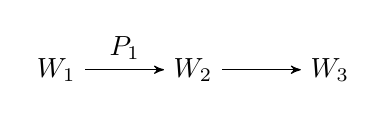
\begin{tikzpicture}[>=stealth']
{[start chain]
\node[on chain] (A) {$W_1$};
\node[on chain,join=by {->,"$P_1$"},right=of A] (B) {$W_2$};
\node[on chain,join=by {->},right=of B] (C) {$W_3$};}
\end{tikzpicture}
\end{center}
The system values are defined as...
\begin{center}
\begin{tabular}{ c|c c c }
& $W_1$ & $W_2$ & $W_3$ \\
\hline 
$h_s(P_{1,yAL})$ & $NULL$ & $NULL$ & $NULL$ \\ 
$h_{sf}(P_{1,yAL})$ & $NULL$ & $NULL$ & $NULL$ \\ 
Neighbor & $W_2$ & $W_1$ \& $W_3$ & $W_1$\\
\end{tabular}
\end{center}

\begin{enumerate}
\item $W_2$ must verify that $P_1$ currently resides in $W_1$, this is done by ensuring $h_{sf}(P_{1,yAL}) = NULL$ this is found by sending a signed data request message from $W_2$ to $W_1$ 
\item $W_2$ insures that $W_1$ is adjasent to itself
\item The player presents a $P_{1,1AL}$ to $W_2$
\item $W_1$ calculates $h_s(P_{1,1AL})$ using the $AL$ on the serverside
\item $W_2$ calculates $h_s(P_{1,1AL})$ using the $AL$ provided by $P_1$, the hashes must match
\item (Optional) The Action ledger traceback can be complete
\item $P_1$ is now granted access to $W_2$ and can submit action 
\item $W_1$ Must store $h_s(P_{1,1AL})$, $P_{1,1AL}$ can be deleted
\end{enumerate}

The network state is now as follows...

\begin{center}
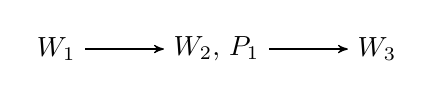
\begin{tikzpicture}[>=stealth']
{[start chain]
\node[on chain] (A) {$W_1$};
\node[on chain,join=by {->},right=of A] (B) {$W_2$, $P_1$};
\node[on chain,join=by {->},right=of B] (C) {$W_3$};}
\end{tikzpicture}
\end{center}
The system values are defined as...
\begin{center}
\begin{tabular}{ c|c c c }
& $W_1$ & $W_2$ & $W_3$ \\
\hline 
$h_s(P_{1,yAL})$ & $ h_s(P_{1,1AL})$ & $NULL$ & $NULL$ \\ 
$h_{sf}(P_{1,yAL})$ & $NULL$ & $NULL$ & $NULL$ \\ 
Neighbor & $W_2$ & $W_1$ \& $W_3$ & $W_1$\\
\end{tabular}
\end{center}

If the player now moves to $W_3$...

\begin{center}
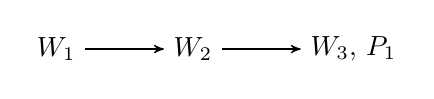
\begin{tikzpicture}[>=stealth']
{[start chain]
\node[on chain] (A) {$W_1$};
\node[on chain,join=by {->},right=of A] (B) {$W_2$};
\node[on chain,join=by {->},right=of B] (C) {$W_3$, $P_1$};}
\end{tikzpicture}
\end{center}
The system values are defined as...
\begin{center}
\begin{tabular}{ c|c c c }
& $W_1$ & $W_2$ & $W_3$ \\
\hline 
$h_s(P_{1,yAL})$ & $h_s(P_{1,1AL})$ & $h_s(P_{1,2AL})$ & $NULL$ \\ 
$h_{sf}(P_{1,yAL})$ & $h_s(P_{1,2AL})$ & $NULL$ & $NULL$ \\ 
Neighbor & $W_2$ & $W_1$ \& $W_3$ & $W_1$\\
\end{tabular}
\end{center}


\subsection{Player Genesis} Is the creation of a new player, for this to occur a player must digitally sign a genesis package with the current nuance of the world. The player is then instated into the world with all the initial player values set to zero. 

\section{Trust}
The system only works if the neighboring worlds trust each other. It's possible for neighboring worlds to have disagreements and still function. For instance, $W_1$ might introduce an item $W_2$ consider to be too powerful, in this case the world can just neglect it's existence, any action presented using that item would be considered illegal and not entered into the action ledger of the $W_1$.

Worlds that have rules that are considered to be completely egregious can be neglected. As an example lets say $W_1$ borders $W_2$ and $W_2$ borders $W_3$, but $W_1$ does not border $W_3$. 

\begin{center}
\begin{tikzpicture}
\draw (0,0) rectangle (3,3) node[pos=.5] {$W_1$}[shift={(-30,0)}];
\end{tikzpicture}
\begin{tikzpicture}
\draw (0,0) rectangle (3,3) node[pos=.5] {$W_2$}[shift={(0,0)}];
\end{tikzpicture}
\begin{tikzpicture}
\draw (0,0) rectangle (3,3) node[pos=.5] {$W_3$}[shift={(30,0)}];
\end{tikzpicture}
\end{center}

It's entirely possible that $W_1$ might not agree with the rules of $W_3$. There are two ways of dealing with a dispute like this, either a world disconnect or Action Ledger Traceback. 

\subsubsection{Action Ledger traceback}
When a player enters a world, the world has the option to traceback the Action ledger of a player to either the last entry in that world, or the players genesis. A world may wish to trust the consensus of the adjacent world, but this is a security question to be answered by the world itself. If the world conducts an action ledger traceback, and the traceback contains actions in a world that are not considered canon by the world doing the audit, the rewards and actions committed in the offending world are neglected in the world doing the audit.

\subsubsection{World Disconnects}
It's possible a world may issue a disconnect of an adjacent world, this means that players can no longer travel back and fourth through these worlds. If the player resided in the disconnected world this could leave the player stranded in the offending world. It would be logical for the world that issued the disconnect to accept the player back into the world in an earlier state before the player moved into the offending world. 


% \begin{center}
% \begin{tikzpicture}
% \draw (0,0) rectangle (1,1) node[pos=.5] {Test};
% \end{tikzpicture}
% \end{center}

\end{document}
